\documentclass[tikz,border=5pt]{standalone}
\usepackage{luatexja}
\usepackage[hiragino-pron]{luatexja-preset}
\usepackage{amsmath,amssymb,bm}
\usetikzlibrary{arrows.meta}

\begin{document}
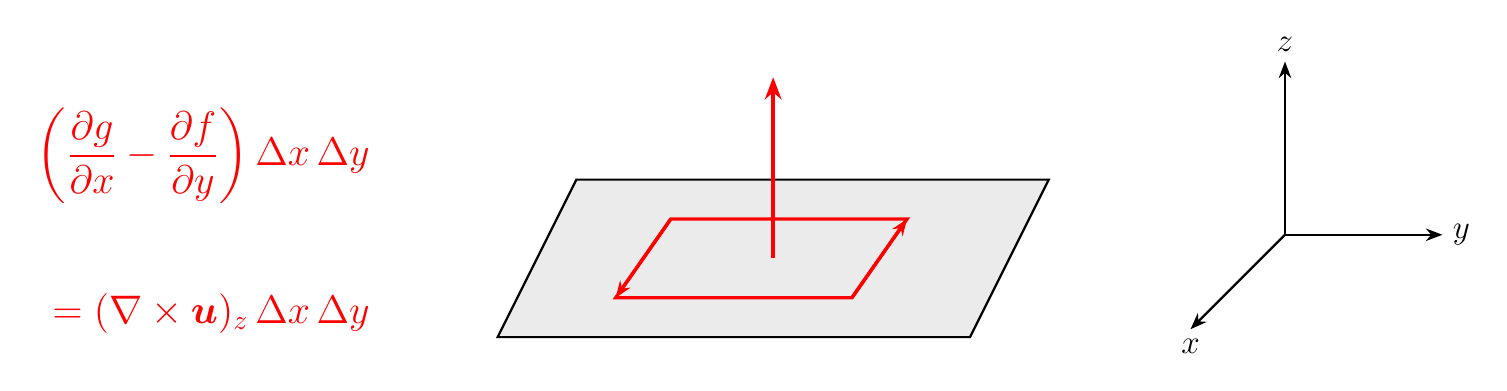
\begin{tikzpicture}[every node/.style={font=\large}]

  %% Left: formula
  \node[red, font=\Large, anchor=east] at (0,1.5) {$\left(\dfrac{\partial g}{\partial x} - \dfrac{\partial f}{\partial y}\right) \Delta x\, \Delta y$};
  \node[red, font=\Large, anchor=east] at (0,-0.5) {$= (\nabla \times \boldsymbol{u})_z\, \Delta x\, \Delta y$};

  %% Center: xy-plane with circulation and z-component arrow
  \begin{scope}[xshift=4.5cm]
    % Parallelogram for xy-plane (perspective view)
    \fill[black!8] (-3,-0.8) -- (3,-0.8) -- (4,1.2) -- (-2,1.2) -- cycle;
    \draw[thick] (-3,-0.8) -- (3,-0.8) -- (4,1.2) -- (-2,1.2) -- cycle;

    % Circulation arrow (red, counterclockwise on the plane)
    \draw[-{Stealth[length=6pt]}, very thick, red]
      (-1.5,-0.3) -- (1.5,-0.3) -- (2.2,0.7) -- (-0.8,0.7) -- cycle;
    \draw[-{Stealth[length=6pt]}, very thick, red]
      (1.5,-0.3) -- (2.2,0.7);
    \draw[-{Stealth[length=6pt]}, very thick, red]
      (-0.8,0.7) -- (-1.5,-0.3);

    % z-component arrow (red, pointing up)
    \draw[-{Stealth[length=8pt]}, ultra thick, red] (0.5,0.2) -- (0.5,2.5);
  \end{scope}

  %% Right: xyz axes
  \begin{scope}[xshift=11.5cm, yshift=0.5cm]
    \draw[-{Stealth[length=6pt]}, thick] (0,0) -- (0,2.2) node[above] {$z$};
    \draw[-{Stealth[length=6pt]}, thick] (0,0) -- (2,0) node[right] {$y$};
    \draw[-{Stealth[length=6pt]}, thick] (0,0) -- (-1.2,-1.2) node[below] {$x$};
  \end{scope}

\end{tikzpicture}
\end{document}
